\documentclass[12pt]{article}
\usepackage{graphicx}
\usepackage[colorlinks=true, pdfborder={0 0 0}, linkcolor=blue, urlcolor=blue, citecolor=blue]{hyperref}
\usepackage[a4paper, margin=.5in]{geometry}
\usepackage{float}
\usepackage{amsmath}

\begin{document}

\title{Lasers}
\author{Sudarsan D Naidu}
\maketitle

\tableofcontents

\section{Introduction}

LASER means \textbf{Light Amplification by Stimulated Emission of Radiation}. To understand the mechanism of Laser, one has to understand the concept of Energy levels (which will be studied later in Quantum Field theory).

\subsection{Energy Level}

An energy level is a specific, quantized state that an $e^{-}$ can occupy in an atom or molecule, each with a fixed energy value. We will be studying about these energy levels in depth when we will be learning Quantum Physics. \vspace{.2cm}

\textbf{What does an atom getting excited mean?} An atom getting excited means that the atom has gained some energy (relative to its ground state). When an electron of the atom get excited, it gains energy and as an electron is part of an atom, so the atom too does gain energy. From whatever we know till now, when a photon is absorbed by an atom, it is more accurate to say that the electron has been excited. But, in this chapter, we will often keep atom as our point of reference. So, whenever we say that an atom has been excited, we refer to excitation of the outermost valence shell electron. Refer to Born-Oppenheimer approximation for a better idea on how nucleus of an atom is not affected when the photon is absorbed by the atom.

\begin{quote}
    If an electron has been excited, then the atom too gets excited but if an atom has been excited, there are many possibilities. But, in this chapter, we will be only considering the excitation of the outermost valence shell electron as the only possibility.
\end{quote}

\subsection{Energy Gap}

Usually for an \textbf{isolated gaseous atom}, there are many energy levels in discrete which the electron can occupy. But, in the case of solids, due to tightly packed atoms and their orbital overlap, the discrete energy levels become very close and appear to be continuous. Such continuous energy levels are called as energy bands and the $e^{-}$ can take any energy value between the lowest and highest value of energy band. The concept of energy bands will be discussed again in Band Theory of Solids in depth.

\subsection{Classical Representation of Atom}

In classical view (an extended version of Newtonian mechanics), these energy levels are related with the orbits of the $e^{-}$ revolving around the nucleus (See figure 1).

\begin{figure}[H]
    \centering
    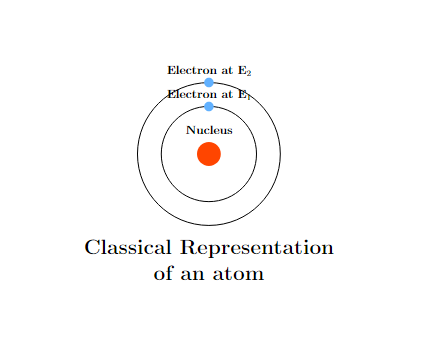
\includegraphics[scale=0.5]{./img/01_classical_atom.png}
    \caption{Classical Representation of an Atom}
\end{figure}

This idea is very outdated and is wrong as we move towards the concept of Quantum Mechanics. The atom is often represented like this in some books to keep things simple. In the quantum mechanical model of the atom, we consider electrons to be in the orbitals corresponding to their energy levels.

\subsection{Energy Level Diagrams}

To explain phenomena related to interaction between radiation and matter, we need a good diagrammatic representation of an atom. As stated earlier, we are not interested in outdated classical representation of atom anymore in favour of the quantum mechanical model. \vspace{.2cm}

Now, if we follow the quantum mechanical model, representing orbitals in an atom is highly complicated, making it even more challenging to use those diagrams to explain certain phenomena. We have discussed earlier that in this chapter we are going to equate energy states of an atom with the energy state of its outermost valence electron, i.e. when an electron excites from $E_{1}$ to $E_{2}$, the atom too excites from $E_{1}$ to $E_{2}$. So, instead of using diagrams of electrons, orbitals or orbits, we will be using the diagram of energy levels (see figure 2) to explain several phenomena.

\begin{figure}[H]
    \centering
    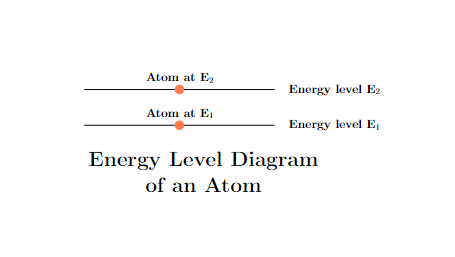
\includegraphics[scale=0.8]{./img/02_energy_levels.png}
    \caption{Energy level diagram of an Atom}
\end{figure}

This energy level diagram helps use to visualise in which energy state the atom (or its outermost valence shell $e^{-}$) is in without violating any idea of quantum mechanical model of an atom. Compare figure 2 with figure 1.

\subsection{References}

\begin{itemize}
    \item Read Basavaraju's book on Engineering Physics for fundamental ideas (Chapter 5 Lasers)
    \item Watch this \href{https://www.youtube.com/watch?v=_JOchLyNO_w&t=233s}{YT video} for a complete animated video of the whole mechanism of LASER. The only con of this video will be its attempt of using the classical representation of atom in it.
    \item See this \href{https://www.reddit.com/r/Physics/comments/1ev7gss/are_energy_levels_for_electrons_or_atoms/}{Reddit post} for question on energy levels.
\end{itemize}

This page has to be updated once we complete studying Quantum Physics and its mechanics.

\section{Types of Interactions}

Working of laser depends on the three different ways of interaction of radiation and matter. In this chapter, there will only be an introduction to the interactions and will study them later in depth in Quantum Mechanics. \textbf{Note} that these interactions happen only in isolated atoms with discrete $E$ levels.

\subsection{Stimulated Absorption}

This interaction is also called as \textbf{Induced Absorption} in some books (like in Basavaraju) while in some others, it is called as \textbf{Stimulated Absorption}.

\begin{figure}[H]
    \centering
    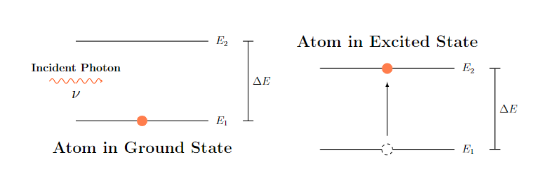
\includegraphics[scale=0.5]{./img/03_induced_absorption.png}
    \caption{Stimulated Absorption}
\end{figure}

Here (and for the other 2 interactions too), assume $E_{1}$ is the ground state and $E_{2}$ is some excited state of that atom.

\begin{equation}
    \Delta E = E_{1} - E_{2}
\end{equation}

Here, the photon is absorbed by the atom to excite itself from the ground state to an excited state. This is only possible if the energy of photon is same as the energy different between two levels. So, by \textbf{Planck's formula}.

\begin{equation}
    \Delta E = h\nu
\end{equation}

\subsection{Spontaneous Emission}

\begin{figure}[H]
    \centering
    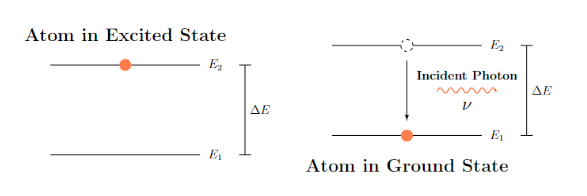
\includegraphics[scale=0.5]{./img/04_spontaneous_emission.png}
    \caption{Spontaneous Emission}
\end{figure}

Any atom in an excited state is unstable and tends to de-excite to the ground state without any external aid (thus spontaneous). During this process, it emits an photon of an energy equal to the energy difference. \textbf{Note} that, there is an universal tendency for any system to be in the lowest energy state to keep itself stable.

Photons emitted by two atoms excited under (and are in) identical conditions undergoing spontaneous emission, \textbf{will not have any phase relationship} (i.e. in any direction and can have phase differences). So, photons emitted under this process are incoherent (i.e. no phase relationship). Such incoherent emissions can be seen in Thermoionic emission in bulb, candle flame, etc.

\subsection{Stimulated Emission}

\begin{figure}[H]
    \centering
    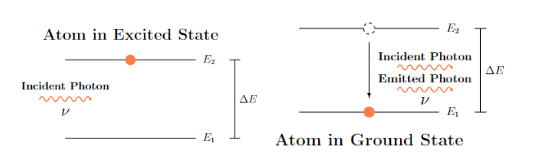
\includegraphics[scale=0.5]{./img/05_stimulated_emission.png}
    \caption{Stimulated Emission}
\end{figure}

Although, atoms can get de-excited without any external aid as seen in Spontaneous emission, they can also get de-excited by an incident photon of an energy equal to the energy difference between the excited levels. When such de-excitation happens, the atom emits another photon which will be in phase (i.e. coherent) with the incident photon. This process is also referred to as "negative absorption".

\section{Einstein's Coefficients}

The formation of atomic spectral lines is due to the three different interactions of radiation and matter which was proposed by Einstein in 1916. Each of these processes are associated with Einstein coefficient, which is a measure of the probability of that particular process occurring. Einstein considered the case of isotropic radiation of frequency $\nu$ (i.e. having same frequency in all directions the radiation is propagating at) and spectral energy density $\rho(\nu)$. \vspace{.2cm}

Read more about this \href{https://en.wikipedia.org/wiki/Einstein_coefficients}{in Wikipedia}.

\subsection{Spectral Energy Density}

Let radiation of continous spectrum of frequencies be incident on the system. Let $\rho(\nu)d\nu$ be the energy incident per unit volume (i.e. energy density) of the radiations having frequencies between $\nu$ and $\nu + d\nu$ in the spectrum. Here, $\rho(\nu)$ is called as spectral energy density (having dimensions of $E/A\nu$) which is the energy density per frequency of radiations having frequencies between $\nu$ and $\nu + d\nu$.

Also, in some books, this has been represented by $U_{\gamma}$ where the frequency is represented by $\gamma$. \textbf{Note} that, this parameter is independent of direction of radiation as we have assumed isotropic frequencies.

\subsection{Population distribution of Atoms in Excited states}

In a system, let $n_{i}$ be the number density (i.e. number of units per unit volume) of atoms existing in the energy state $i$. To keep things more simple in understanding the lasing process, we will use the energy level diagrams to show the distribution of atoms of system in the excited states (see figure 6).

\begin{figure}[H]
    \centering
    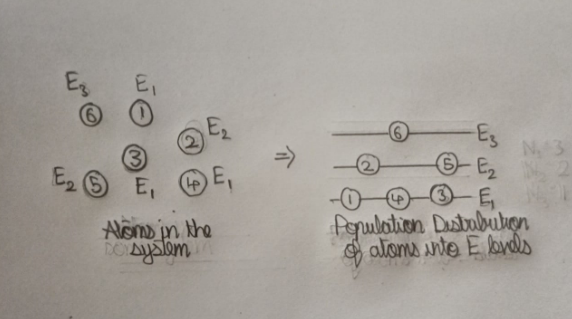
\includegraphics[scale=.5]{./img/06_population_dist.png}
    \caption{Population distribution of atoms of the system into their respective energy states}
\end{figure}

Then, $dn_{i}/dt$ will be the rate at which the number density of atoms exciting or de-exciting (depending on the sign of the derivative) to an energy state $i$. 

Let's consider a system having energy states $E_{1}$, $E_{2}$, ..., $E_{i}$. Let it have a total population density (of atoms) $n$,

\begin{equation}
    n_{1} + n_{2} + ... + n_{i} = n
\end{equation}

We can differentiate this equation (w.r.t $t$) to get a relation between the rate of atoms exciting and de-exciting in each energy state,

\begin{equation*}
    \frac{dn_{1}}{dt} + \frac{dn_{2}}{dt} + ... + \frac{dn_{i}}{dt} = \frac{dn}{dt}
\end{equation*}

In a fixed system, we can assume $n$ to be constant, which makes $dn/dt$ to be 0,

\begin{equation*}
    \frac{dn_{1}}{dt} + \frac{dn_{2}}{dt} + ... + \frac{dn_{i}}{dt} = 0
\end{equation*}

In transition of atoms, involving only two states, the rates of other states will become zero,

\begin{align}
    \frac{dn_{1}}{dt} + \frac{dn_{2}}{dt} & = 0 \notag \\
    \Rightarrow \frac{dn_{2}}{dt} & = -\frac{dn_{1}}{dt}
\end{align}

\subsection{Description of Einstein's coefficients}

Let's consider two energy levels $E_{1}$ (ground state) and $E_{2}$ (some excited state) where $n_{1}$ and $n_{2}$ are the respective population densities of atoms in those energy states. Now, let's see how the three kinds of interactions of radiation and matter are described by the Einstein's coefficients,

\subsubsection{Stimulated Absorption}

In this process, the atoms excite from $E_{1}$ to $E_{2}$ due to the incident radiation of frequency $\nu$. To measure the rate of this process (and for the others too), we will consider $E_{1}$ (ground state) and its population density $n_{1}$ as reference, i.e.,
\begin{align*}
    \text{Rate of stimulated} & = \text{Rate at which atoms are undergoing stimulated} \\
    \text{absorption} & \quad \text{absorption from } E_{1} \text{ to } E_{2} \\ 
    & = (\frac{dn_{1}}{dt})_{s.a.}
\end{align*}

And, from experiments, we know, 
\begin{align*}
    \textnormal{Rate of stimulated absorption} \propto -n_{1}\rho(\nu) \\ 
    (\frac{dn_{1}}{dt})_{s.a.} \propto -n_{1}\rho(\nu)
\end{align*}

As atoms excite from $E_{1}$ to $E_{2}$, it results in decrease in $n_{1}$ (and increase in $n_{2}$) which explains the negative sign. The rate of stimulated absorption will be more if there are more atoms in the ground state $E_{1}$ to get excited to $E_{2}$ so the rate depends on $n_{1}$. This points out the fact that the rate of stimulated absorption will decrease as more and more atoms in $E_{1}$ get excited. Also, as this process is initiated by the energy of the incident radiation, it also depends on the spectral energy density of it. \vspace{.2cm}

The proportional constant for the equation is the Einstein coefficient $B_{12}$ where $12$ shows the direction of process (i.e. $E_{1}$ to $E_{2}$). After plugging the Einstein coefficient in the proportional equation, we get,

\begin{equation}
    (\frac{dn_{1}}{dt})_{s.a.} = -B_{12}n_{1}\rho(\nu) 
\end{equation}

To find the rate at which the atoms are getting excited to $E_{2}$ by stimulated absorption, we can substitute the above rate in the equation (4),

\begin{equation*}
    (\frac{dn_{2}}{dt})_{s.a.} = -(\frac{dn_{1}}{dt})_{s.a.} = B_{12}n_{1}\rho(\nu)
\end{equation*}

\subsubsection{Spontaneous Emission}

In this process, the atoms de-excite from $E_{2}$ to $E_{1}$ spontaneously (i.e. without any external aid). Like we did for stimulated absorption, we are going to consider $E_{1}$ (ground state) as our reference to find rate of this emission.
\begin{align*}
    \text{Rate of spontaneous} & = \text{Rate at which atoms are undergoing spontaneous} \\
    \text{emission} & \quad \text{emission from } E_{2} \text{ to } E_{1} \\ 
    & = (\frac{dn_{1}}{dt})_{sp.e.}
\end{align*}

And, from experiments, we know, 
\begin{align*}
    \textnormal{Rate of spontaneous emission} \propto n_{2} \\ 
    (\frac{dn_{1}}{dt})_{sp.e.} \propto n_{2}
\end{align*}

As atoms de-excite from $E_{2}$ to $E_{1}$, there will be an increase in $n_{1}$ which explains why it has no negative sign. The rate of spontaneous emission will be more if there are more excited atoms in $E_{2}$ (i.e. $n_{2}$) to get de-excited spontaneously, so the rate depends on $n_{2}$. As this process is independent of any external aid (i.e. no incident radiation like in stimulated absorption), the rate is independent of spectral energy density. \vspace{.2cm}

The proportional constant for the equation is the Einstein coefficient $A_{21}$ where $21$ shows the direction of process (i.e. $E_{2}$ to $E_{1}$). After plugging the Einstein coefficient in the proportional equation, we get,
\begin{equation}
    (\frac{dn_{1}}{dt})_{sp.e.} = B_{21}n_{2}
\end{equation}

We can get the rate of this emission keeping $E_{2}$ as our reference by applying equation (4) like we did earlier in stimulated absorption.

\subsubsection{Stimulated Emission}

In this process, the atoms de-excite from $E_{2}$ to $E_{1}$ due to incident of radiation of frequency $\nu$. Taking $E_{1}$ (ground state) as our reference like we did earlier.
\begin{align*}
    \text{Rate of spontaneous} & = \text{Rate at which atoms are undergoing spontaneous} \\
    \text{emission} & \quad \text{emission from } E_{2} \text{ to } E_{1} \\ 
    & = (\frac{dn_{1}}{dt})_{s.e.}
\end{align*}

And, from experiments, we know, 
\begin{align*}
    \textnormal{Rate of spontaneous emission} \propto n_{2} \\ 
    (\frac{dn_{1}}{dt})_{s.e.} \propto n_{2}
\end{align*}

\end{document}